% Template for Seminar Papers
% Research Group for Parallel Computing
% Vienna University of Technology

% Copyright (C) 2015-2016
% Sascha Hunold <hunold@par.tuwien.ac.at>
% version 1.0.2

\documentclass[DIV12,a4paper]{scrartcl}

\usepackage[utf8]{inputenc}
\usepackage[T1]{fontenc}

%\usepackage{fixltx2e} 
\usepackage{amsmath}  
\usepackage{amssymb} 
\usepackage{microtype} 
\usepackage{enumitem} 
\usepackage{booktabs} 
\usepackage{nag}       % Issues warnings when best practices in writing LaTeX documents are violated.
\usepackage{hyperref}
\usepackage{xspace}
\usepackage{graphicx}

%custom packages
\usepackage[backend=biber,style=ieee]{biblatex}

%%%%%%%%%%%%%%%%%%%%%%%%%%%%%%%%%%%
% ONLY CHANGE THE FOLLOWING MACROS

% your name
\newcommand{\studname}{Stefan Haider}

% your matrikel
\newcommand{\studmatrikel}{1125543}

% name of seminar
\newcommand{\seminarname}{Efficient Shared Memory Programming}

% title of your seminar paper
\newcommand{\seminartitle}{The Adaptive Priority Queue with Elimination and Combining}

% date when you hand in seminar paper
\newcommand{\spdate}{24. Feb. 2017}

% uncomment your choice
\newcommand{\sptopic}{Seminar aus Programmiersprachen}
%\newcommand{\sptopic}{Seminar aus Algorithmik}
%\newcommand{\sptopic}{Seminar aus Software Engineering}
%\newcommand{\sptopic}{Seminar aus Theoretischer Informatik}

% who is supervising
\newcommand{\spbetreuer}{Univ.Prof. Dr. Jesper Larsson Träff}

% YOU SHOULD NOT NEED TO CHANGE THE REMAINING FILE
%%%%%%%%%%%%%%%%%%%%%%%%%%%%%%%%%%%

%custom configuration
\addbibresource{progsem.bib}

\graphicspath{{graphics/}}

\begin{document}

% !TEX root = ../paper.tex

\pagestyle{empty}

\begin{titlepage}
\begin{center}

\includegraphics[scale=1]{TU_INF_Logo_gray}
\hfill

\includegraphics[width=1.7cm]{final-logo-par}

\end{center}

\vspace*{1cm}

\begin{center}

\begin{Large}
Institut für Informationssysteme\\
Forschungsgruppe ``Parallel Computing'' (E184-5)\\
Prof. Dr. Jesper Larsson Träff\\[2cm]
\end{Large}

\begin{Huge}
\textbf{Seminararbeit}\\
\end{Huge}

\vspace*{1cm}

\begin{Large}
für ein \\
\sptopic{} \\
``\seminarname{}'' 
\end{Large}


\vspace*{2cm}

\begin{Large}
\textbf{``\seminartitle{}''}
\end{Large}

\vspace*{2cm}

\begin{Large}
\studname \\
Matrikelnummer: \studmatrikel\\[2cm]

Betreuer: \spbetreuer

\vspace*{2cm}
\spdate \\

\end{Large}
\end{center}

\end{titlepage}


\cleardoublepage


\section*{Main Literature Sources}

The following seminar report is based on the following research articles:

% CHANGE THIS LIST ACCORDINGLY

\begin{itemize}
\item Ambuj K. Singh, James H. Anderson, Mohamed G. Gouda: The Elusive Atomic Register. J. ACM (JACM) 41(2):311-339 (1994)
\item Danny Dolev, Nir Shavit: Bounded Concurrent Time-Stamping. SIAM J. Comput. 26(2): 418-455 (1997)
\end{itemize}


\clearpage

\section*{Erkl\"arung zur Verfassung der Arbeit}

\vspace*{3ex}

\noindent
Hiermit erkl\"are ich, dass ich diese Arbeit selbst\"andig verfasst habe, dass ich die verwendeten Quellen und Hilfsmittel vollst\"andig angegeben habe und dass ich die Stellen der Arbeit -- einschließlich Tabellen, Karten und Abbildungen --, die anderen Werken oder dem Internet im Wortlaut oder dem Sinn nach entnommen sind, auf jeden Fall unter Angabe der Quelle als Entlehnung kenntlich gemacht habe.\\[5ex]

\noindent
\rule{8cm}{.5pt} \\
Wien, \spdate \\
\studname


\clearpage

\tableofcontents

\cleardoublepage

\pagestyle{plain}

\setcounter{page}{1}

% !TEX root = ../paper.tex

\section{Introduction}

Here goes the introduction. We also cite the nice book of Pinedo~\cite{calciu_adaptive_2014,bar-nissan_dynamic_2011,hendler_flat_2010,lotan_skiplist-based_2000,sundell_fast_2003}.

\section{Algorithm X}

Table~\ref{tab:related_algorithms} shows a summary of related algorithms.

\begin{table}[t]
\centering
\captionabove{Related algorithms and their complexity.}
\label{tab:related_algorithms}
\begin{tabular}{ll}
\toprule 
algorithm & complexity \\
\midrule
algorithm Y & $O(n)$ \\
algorithm Z & $O(n \log{n} )$ \\
\bottomrule
\end{tabular}
\end{table}

\section{Evaluation of Algorithm X}

The run-time of our algorithm is shown in Figure~\ref{fig:runtime}.

\begin{figure}[t]
\centering
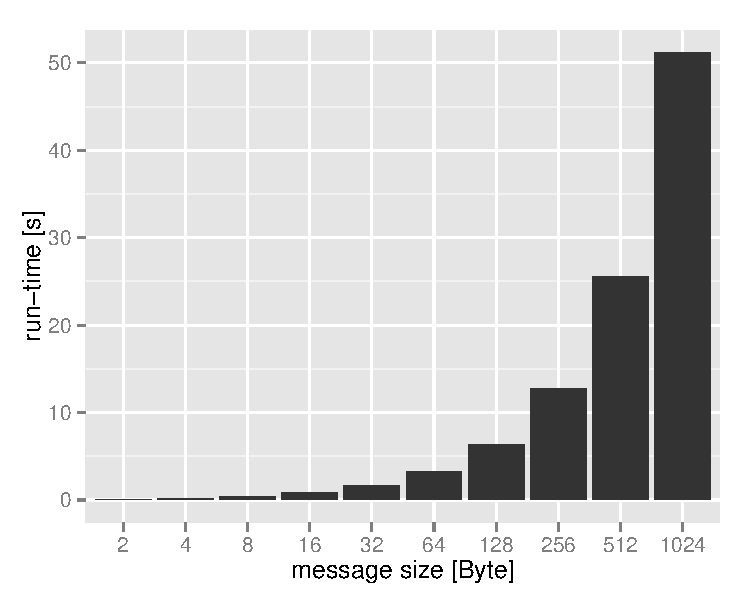
\includegraphics[width=.5\linewidth]{figures/runtime}
\caption{Run-time of algorithm X on machine Y.}
\label{fig:runtime}
\end{figure}

\section{Summary}
We summary the contribution of the papers and this seminar paper.


\cleardoublepage
% Add a bibliography
%\bibliographystyle{plain}
\printbibliography

\end{document}